\documentclass{article}
\usepackage{amsfonts}
\usepackage{amsmath}
\usepackage{amsthm}
\usepackage{hyperref}
\usepackage{graphicx}
\usepackage{cleveref}
\usepackage{txfonts}
\usepackage{minted}

\begin{document}
\section{Neural Networks and Deep Learning}
See \url{https://www.deeplearning.ai/} for the course.
\subsection{Introduction}
Machine learning has different applications
\begin{itemize}
\item real estate, online advertising (standard neural networks)
\item image classification (CNN)
\item audio to text, language translation (RNN)
\item position of other cars in autonomous driving (hybrid)
\end{itemize}

Supervised learning uses data consisting of input (x) and desired output (y).
In supervised learning there is structured data (house price and features)
and unstructured data (images, audio, text).

Traditional approaches hit a performance plateau as more and more data becomes available.
Deep learning is facilitated by
\begin{itemize}
\item larger datasets
\item more computational power
\item algorithmic improvements
\end{itemize}

Geoffrey Hinton's advice:
\begin{itemize}
\item read enough so that you start developing intuitions
\item trust your intuitions
\item never stop programming
\end{itemize}

\subsection{Basics of Neural Network programming}
\subsubsection{Binary Classification}
Logistic regression is an algorithm for binary classification (e.g. y=1 (cat) vs y=0 (no cat)).
The training set consists of samples $(x,y)$ with $x\in\mathbb{R}^{n_x}$ and $y\in\{0,1\}$.
The training set is $(x^{(1)},y^{(1)}), (x^{(2)},y^{(2)}), \ldots, (x^{(m)},y^{(m)})$ with $m=m_{train}$ (or $m=m_{test}$ for the test set).
The training data is represented by the matrix
\begin{equation}
  X=\begin{pmatrix}x^{(1)} & x^{(2)} & \cdots & x^{(m)}\end{pmatrix}\in\mathbb{R}^{n_x\times m}
\end{equation}
The labels are
\begin{equation}
  Y=\begin{pmatrix}y^{(1)} & y^{(2)} & \cdots & y^{(m)}\end{pmatrix}\in\mathbb{R}^{1\times m}
\end{equation}

Logistic regression tries to model the probability $\widehat{y}=P(y=1|x)$.
The model has the parameters $w\in\mathbb{R}^{n_x}$ and $b\in\mathbb{R}$.
The model is $\widehat{y}^{(i)}=\sigma(w^\top x^{(i)}+b)$ using $\sigma(z^{(i)})=\frac{1}{1+e^{-z^{(i)}}}$.
Also see \cref{fig:sigmoid}.
\begin{figure}[htbp]
  \begin{center}
    \includegraphics[width=.5\textwidth]{sigmoid}
    \caption{The sigmoid activation function}
    \label{fig:sigmoid}
  \end{center}
\end{figure}

\subsubsection{Cost function}
The logistic regression \emph{loss function} computes the error for a single training example.
\begin{equation}
  \mathcal{L}(\widehat{y},y)=-\big(y\log\widehat{y}+(1-y)\log(1-\widehat{y})\big)
\end{equation}
with $y\in\{0,1\}$.
The \emph{cost function} is the average of the loss function of the entire training set.
\begin{equation}
  J(w,b)=\frac{1}{m}\sum_{i=1}^m\mathcal{L}(\widehat{y}^{(i)},y^{(i)})=
  -\frac{1}{m}\sum_{i=1}^m\big[y^{(i)}\log\widehat{y}^{(i)}+(1-y^{(i)})\log(1-\widehat{y}^{(i)})\big]
\end{equation}

\subsubsection{Gradient descent}
Gradient descent iteratively minimizes $J(w,b)$ using partial derivatives of $J$.
\begin{equation}
  \begin{split}
    w&\coloneqq w-\alpha\underbrace{\frac{\partial J(w,b)}{\partial w}}_{\eqqcolon dw}\\
    b&\coloneqq b-\alpha\underbrace{\frac{\partial J(w,b)}{\partial b}}_{\eqqcolon db}
  \end{split}
\end{equation}
$\alpha$ is the learning rate.

Derivative chain-rule: $\frac{df(g(x))}{dx}=\frac{df}{dg}\frac{dg}{dx}$.
In the source code $\frac{dJ}{dv}$ is named ``dv'' where $J$ is the final output variable.

In the case of logistic regression with two features $z=w_1x_1+w_2x_2+b$ and $a=\sigma(z)$.
\begin{equation}
  \begin{split}
    \frac{d\mathcal{L}(a,y)}{da}&=-\frac{y}{a}+\frac{1-y}{1-a}\\
    \frac{da}{dz}&=a(1-a)\\
    ``dz''=\frac{d\mathcal{L}}{dz}&=\frac{d\mathcal{L}}{da}\frac{da}{dz}=a-y
  \end{split}
\end{equation}
$\frac{d\mathcal{L}}{dw_1}=``dw_1''=x_1 dz$, $``dw_2''=x_2dz$, and $``db''=dz$.
The update rule for gradient descent then is
\begin{equation}
  \begin{split}
    w_1&\coloneqq w_1-\alpha dw_1\\
    w_2&\coloneqq w_2-\alpha dw_2\\
    b&\coloneqq b-\alpha db\\
  \end{split}
\end{equation}

\subsubsection{Logistic regression on $m$ examples}
Logistic regression over multiple training examples works by simply summing up the derivatives.
\begin{equation}
  \frac{\partial}{\partial w_1}J(w,b)=\frac{1}{m}\sum_{i=1}^m\underbrace{\frac{\partial}{\partial w_1}\mathcal{L}(a^{(i)},y^{(i)})}_{dw_1^{(i)}}
\end{equation}
See \cref{fig:logistic-regression} for more detail.
\begin{figure}
  \begin{center}
    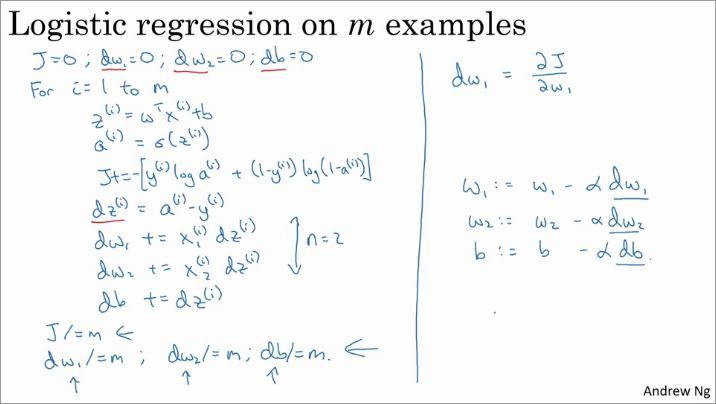
\includegraphics[width=\textwidth]{logistic-regression}
    \caption{Logistic regression on $m$ examples}
    \label{fig:logistic-regression}
  \end{center}
\end{figure}

\subsubsection{Vectorizing Logistic Regression}
\begin{minted}{python}
# Examples for vectorized code
import numpy as np
u = np.dot(A, v)
u = np.exp(v)
np.log(v)
np.maximum(v, o)
v ** 2
\end{minted}

\begin{equation}
  Z=\begin{bmatrix}z^{(1)} & z^{(2)} & \cdots & z^{(m)}\end{bmatrix}=
    w^\top X + \underbrace{\begin{bmatrix}b & b & \cdots & b\end{bmatrix}}_{\in\mathbb{R}^{1\times m}}
\end{equation}

In Python:
\begin{minted}{python}
  Z=np.dot(w.T, x)+b
\end{minted}

\begin{equation}
  A=\begin{bmatrix}a^{(1)} & a^{(2)} & \cdots & a^{(m)}\end{bmatrix}=\sigma(Z)
\end{equation}

\begin{equation}
  dZ=\begin{bmatrix}dz^{(1)} & dz^{(2)} & \cdots & dz^{(m)}\end{bmatrix}
\end{equation}

\begin{equation}
  dZ=A-Y
\end{equation}

\begin{equation}
  db=\frac{1}{m}\sum_{i=1}^m dz^{(i)}
\end{equation}

\begin{minted}{python}
A = sigmoid(np.dot(w.T, X) + b)
cost = -np.sum(Y * np.log(A) + (1 - Y) * np.log(1 - A)) / m
dw = np.dot(X, (A - Y).T) / m
db = np.sum(A - Y) / m
\end{minted}

\begin{equation}
  dw=\frac{1}{m}X dz^\top
\end{equation}

\begin{equation}
  \begin{split}
    w &\coloneqq w-\alpha dw\\
    b &\coloneqq b-\alpha db
  \end{split}
\end{equation}

\subsubsection{Logistic Regression Cost Function}
The two cases
\begin{itemize}
  \item if $y=1$: $p(y|x)=\widehat{y}$
  \item if $y=0$: $p(y|x)=1-\widehat{y}$
\end{itemize}
can be expressed as one equation: $p(y|x)=\widehat{y}^y(1-\widehat{y})^{(1-y)}$.
Then
\begin{equation}
  \log p(y|x)=y\log\widehat{y}+(1-y)\log(1-\widehat{y})
\end{equation}

Overall log-probability to maximise (maximum likelihood)
\begin{equation}
  \log\prod_{i=1}^m p(y^{(i)}|x^{(i)})=\sum_{i=1}^m \underbrace{\log p(y^{(i)}|x^{(i)})}_{-\mathcal{L}(y^{(i)}|x^{(i)})}
\end{equation}
I.e. minimize the negative value
\begin{equation}
  J(w,b)=\frac{1}{m}\sum_{i=1}^m \mathcal{L}(y^{(i)}|x^{(i)})
\end{equation}
which is the cost function.

Interview with Pieter Abbeel on reinforcement learning applied to robotics.

\subsection{One hidden layer Neural Network}
\subsubsection{Neural Network Overview}
\begin{equation}
  \begin{split}a
    z&=w^\top x+b\\
    a&=\sigma(z)\\
    \mathcal{L}(a,y)&=-y\log(a)-(1-y)\log(1-a)
  \end{split}
\end{equation}

In a neural network with one hidden layer we have:
\begin{equation}
  \begin{split}
    z^{[1]}&=W^{[1]}x+b^{[1]}\\
    a^{[1]}&=\sigma(z^{[1]})\\
    z^{[2]}&=W^{[2]}a^{[1]}+b^{[2]}\\
    a^{[2]}&=\sigma(z^{[2]})\\
    \mathcal{L}(a^{[2]},y)&=-y\log(a^{[2]})-(1-y)\log(1-a^{[2]})
  \end{split}
\end{equation}

\subsubsection{Neural Network Representation}
There is
\begin{itemize}
  \item an input layer $a^{[0]}=x$ ($x_1, x_2, \ldots)$
  \item zero, one, or more hidden layer(s) $a^{[l]}$ with $l\in\{1,2,\ldots,L-1\}$
  \item an output layer $\widehat{y}=a^{[L]}$
\end{itemize}
Only the input layer is not counted, \emph{e.g.} a 2 layer neural network has 1 hidden layer.
\begin{equation}
  W^{[l]}=
  \begin{pmatrix}
  w^{[l]\top}_1\\
  w^{[l]\top}_2\\
  \vdots
  \end{pmatrix}
\end{equation}

\subsubsection{Vectorizing across multiple examples}
\begin{equation}
  \begin{split}
    x^{(1)}&\to a^{[L](1)}=\widehat{y}^{(1)}\\
    x^{(2)}&\to a^{[L](2)}=\widehat{y}^{(2)}\\
    &\vdots\\
    x^{(m)}&\to a^{[L](m)}=\widehat{y}^{(m)}
  \end{split}
\end{equation}
The computation of multiple training examples is vectorized using
\begin{equation}
  X=\begin{pmatrix}x^{(1)} & x^{(2)} & \cdots & x^{(m)}\end{pmatrix}\in\mathbb{R}^{n_x\times m}
\end{equation}
(by stacking vectors horizontally) as follows
\begin{equation}
  \begin{split}
    Z^{[1]}&=W^{[1]}X+b^{[1]}\\
    A^{[1]}&=\sigma(Z^{[1]})\\
    Z^{[2]}&=W^{[2]}A^{[1]}+b^{[2]}\\
    A^{[2]}&=\sigma(Z^{[2]})
  \end{split}
\end{equation}

\subsubsection{Activation Functions}
\begin{itemize}
  \item $\sigma(z)=\frac{1}{1+e^{-z}}\in[0,1]$
  \item $\tanh z=\frac{e^z-e^{-z}}{e^z+e^{-z}}\in[-1,1]$
  \item $\operatorname{ReLU}(z)=\max(0, z)$
\end{itemize}

The $\tanh$ function generally is better than $\sigma$ because the mean of the output is zero.
One exception is the output layer where inputs between zero and one are desirable.

\subsubsection{Derivatives of Activation Functions}
\begin{equation}
  g(z)=\frac{1}{1+e^{-z}}\to g^\prime(z)=g(z)(1-g(z))
\end{equation}
\begin{equation}
  g(z)=\tanh{z}\to g^\prime(z)=1-\big(g(z)\big)^2
\end{equation}
\begin{equation}
  g(z)=\max(0, z)\to g^\prime(z)=\left\{\begin{array}{ll}0&\mathrm{\ if\ }z<0\\1&\mathrm{\ if\ }z>0\end{array}\right.
\end{equation}

\subsubsection{Gradient descent for neural networks}
Forward propagation:
\begin{equation}
  \begin{split}
    Z^{[1]}&=W^{[1]}X+b^{[1]}\\
    A^{[1]}&=g^{[1]}(Z^{[1]})\\
    Z^{[2]}&=W^{[2]}A^{[1]}+b^{[2]}\\
    A^{[2]}&=g^{[2]}(Z^{[2]})=\sigma(Z^{[2]})
  \end{split}
\end{equation}
Backpropagation:
\begin{equation}
  \begin{split}
    dZ^{[2]}&=A^{[2]}-Y\\
    dW^{[2]}&=\frac{1}{m}dZ^{[2]}A^{[1]\top}\\
    db^{[2]}&=\frac{1}{m}\sum_i dZ^{[2](i)}\\
    dZ^{[1]}&=W^{[2]\top}dZ^{[2]}*g^{[1]\prime}(Z^{[1]})\\
    dW^{[1]}&=\frac{1}{m}dZ^{[1]}X\\
    db^{[1]}&=\frac{1}{m}\sum_i dZ^{[1](i)}
  \end{split}
\end{equation}
where ``*'' denotes the elementwise product.

\subsubsection{Random Initialization}
Initializing the weights of a neural network to zero is not sufficient.
The activations will be the same.
By initializing the weights randomly, one can ensure that they are linear independent.
\emph{I.e.} it is necessary to break the symmetry.
Usually the weights are initialised to small random values using a Gaussian random distribution with \emph{e.g.} $\sigma=0.01$.
The bias units can be initialised to zero.

Interview with Ian Goodfellow (Generative Adversarial Neural Networks).
His advice: apply the knowledge to something you are interested in, while learning from the book/online lectures.

\subsection{Deep Neural Networks}
Logistic regression is a ``shallow'' neural network.
A neural network with 5 layers can be called a ``deep'' neural network.
\begin{itemize}
  \item $L$ is the number of layers.
  \item $n^{[l]}$ is the number of units in layer $l$.
  \item $n^{[0]}=n_x$ is the number of input units.
  \item $a^{[l]}=g^{[l]}(z^{[l]})$ is the activation at layer $l$
  \item $a^{[0]}=x$ is the input
  \item $a^{[L]}=\widehat{y}$ is the output
  \item $z^{[l]}=W^{[l]}a^{[l-1]}+b^{[l]}$
\end{itemize}

\subsubsection{Forward propagation in a deep network}
\begin{equation}
  \begin{split}
    z^{[1]}&=W^{[1]}x+b^{[1]}\\
    a^{[1]}&=g^{[1]}(z^{[1]})\\
    z^{[2]}&=W^{[2]}a^{[1]}+b^{[2]}\\
    a^{[2]}&=g^{[2]}(z^{[2]})\\
    &\vdots\\
    z^{[L]}&=W^{[L]}a^{[L-1]}+b^{[L]}\\
    \widehat{y}&=g^{[L]}(z^{[L]})
  \end{split}
\end{equation}
Using $a^{[0]}=x$ and $a^{[L]}=\widehat{y}$ one can write in general:
\begin{equation}
  \begin{split}
    z^{[l]}&=W^{[l]}a^{[l-1]}+b^{[l]}\\
    a^{[l]}&=g^{[l]}(z^{[l]})
  \end{split}
\end{equation}
The vectorized form for a training set (by stacking training examples horizontally):
\begin{equation}
  \begin{split}
    Z^{[l]}&=W^{[l]}A^{[l-1]}+b^{[l]}\\
    A^{[l]}&=g^{[l]}(Z^{[l]})
  \end{split}
\end{equation}

\subsubsection{Getting your matrix dimensions right}
The matrix dimensions are as follows:
\begin{itemize}
  \item $W^{[l]}\in\mathbb{R}^{n^{[l]}\times n^{[l-1]}}$
  \item $b^{[l]}\in\mathbb{R}^{n^{[l]}\times 1}$
  \item $z^{[l]},a^{[l]},dz^{[l]},da^{[l]}\in\mathbb{R}^{n^{[l]}\times 1}$
  \item $Z^{[l]},A^{[l]},dZ^{[l]},dA^{[l]}\in\mathbb{R}^{n^{[l]}\times m}$
\end{itemize}

\subsubsection{Why deep representations}
Using the example of learning $x_1\operatorname{xor}x_2\operatorname{xor}\ldots x_n$ one can show that
it can be represented using a deep neural network with $O(\log n)$ layers and $O(n)$ units.
When using only one hidden layer, $O(2^n)$ units are required.

\subsubsection{Building blocks of of deep neural networks}
See \cref{fig:deepblocks}.
\begin{figure}[htbp]
  \begin{center}
    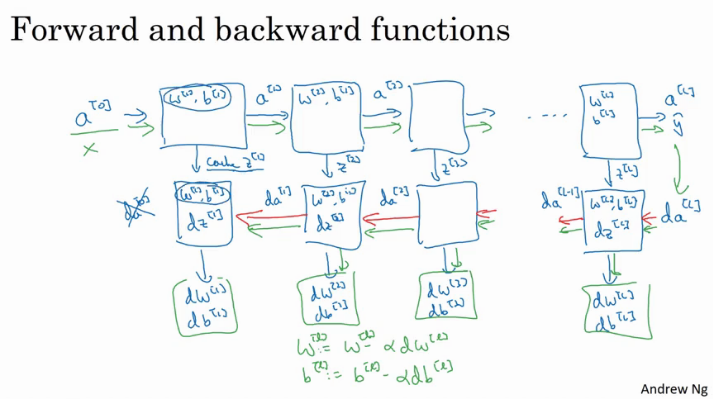
\includegraphics[width=\textwidth]{deepblocks}
    \caption{Building blocks of deep neural network}
    \label{fig:deepblocks}
  \end{center}
\end{figure}

\section{Improving Deep Neural Networks: Hyperparameter tuning, Regularisation}
\section{Structuring Machine Learning Projects}
\section{Convolutional Neural Networks}
\section{Sequence Models}

\end{document}
